\chapter{\SYSTEM{} System Design} \label{sec:design}

\SYSTEM{} acts as a translation layer sitting between the disk and the
operating system. It provides confidentiality and integrity guarantees
while minimizing performance loss due to metadata management overhead.
\SYSTEM{} accomplishes this by leveraging the speed of stream ciphers
over the AES block cipher and taking advantage of the append-mostly
nature of Log-Structured Filesystems (LFS) and modern Flash
Translation Layers (FTL)~\cite{SSD}.

Hence, there are several locations where \SYSTEM{} could be
implemented in the system stack. \SYSTEM{} could be integrated into an
LFS filesystem module itself---\eg{} F2FS---specifically leveraging
the flexibility of the Virtual Filesystem Switch (VFS). \SYSTEM{}
could be implemented as an actual block device or virtual block device
layered atop a physical block device, which is where we chose to
implement our prototype. \SYSTEM{} could even be implemented within
the on-disk SSD controller responsible for managing the flash
translation layer (scatter gather, garbage collection, wear-leveling,
etc.) on modern SSDs and other types of non-volatile storage.

\begin{figure}[ht]
 \centering
  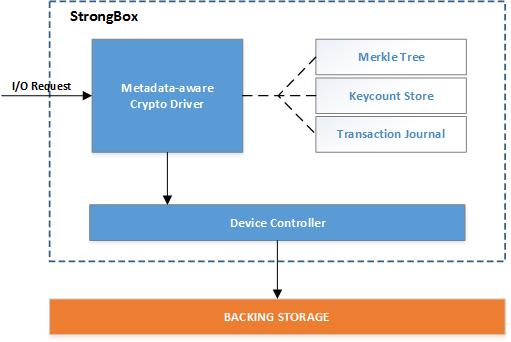
\includegraphics[width=1.0\linewidth]{overview.jpg}
   \caption{Overview of the \SYSTEM{} construction.}
    \label{fig:overview}
\end{figure}

\SYSTEM{}'s design is illustrated in \figref{overview}. \SYSTEM{}'s
metadata is encapsulated in three primary components: an in-memory
\emph{Merkle Tree} and two disk-backed byte arrays, the \emph{Keycount
  Store} and the \emph{Transaction Journal}. These components are
integrated into the \emph{Cryptographic Driver}, which is responsible
for handling data encryption, verification, and decryption during
interactions with the underlying backing store. These interactions
take place while fulfilling high-level I/O requests received from the
overlying LFS. Low-level I/O between \SYSTEM{} and the backing store
is handled by the \emph{Device Controller}.

The rest of this section describes the components referenced in
\figref{overview}. Specifically: we first describe the backing store
and \SYSTEM{}'s layout for data and metadata. This is followed by an
exploration of the cryptographic driver and how it interacts with that
metadata, the role of the device controller, an overview of rekeying
in the backing store, and further considerations to ensure
confidentiality in the case of rollbacks and related attacks.

\section{Backing Store Function and Layout}

% What is it?
The backing store is the storage media on which \SYSTEM{} operates.
\figref{backstore} illustrates \SYSTEM{}'s layout in the backing
store.

\begin{figure}[ht]
 \centering
  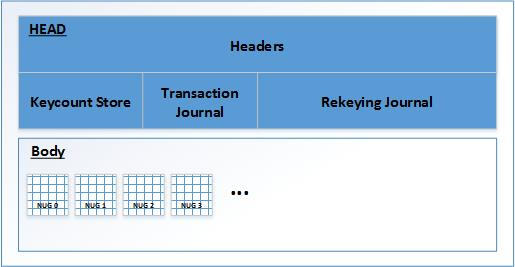
\includegraphics[width=1.0\linewidth]{backstore.jpg}
   \caption{Layout of \SYSTEM{}'s backing storage.}
    \label{fig:backstore}
\end{figure}

% Why is it a thing?
In the \textit{Body} section of the backing store layout, end-user
data is partitioned into a series of same-size logical
\emph{blocks}---distinct from the concept of physical disk blocks,
which are collections of one or more disk sectors. To make this
distinction clear, we refer to these wider logical blocks as
\emph{nuggets}, marked \textit{NUG} in the Body section of
\figref{backstore}. Hence, a nugget consists of one or more physical
disk blocks, depending on its configured size. Each nugget is
subdivided into a constant number of sub-blocks we refer to as
\emph{flakes}. \PUNT{The size of each flake and the number of flakes
  per nugget is configured by the user when \SYSTEM{} is initialized.}

The reason for these nugget/flake divisions are two-fold:
\begin{enumerate}
\item To limit the maximum length of any plaintexts operated on by the
  cryptographic driver, decreasing the overhead incurred per I/O
  operation and
\item To track, detect, and handle overwrites in the backing store.
\end{enumerate}

% Describe how the components in fig 1 are represented on disk and how
% they play into the overall design WITHOUT naming them
Hence, we must keep track of writes so that we may detect when an
overwrite occurs. Flakes are key to this tracking. When a request
comes in to write to one or more flakes in a nugget, \SYSTEM{} marks
the affected flakes ``dirty''. Here, dirty implies that another write
to some portion of that flake would constitute an overwrite. If a new
request comes in to write to one or more of those same flakes another
time, \SYSTEM{} triggers a rekeying procedure over the entire nugget
to safely overwrite the old data in those flakes. This rekeying
procedure is necessarily time consuming, adding to the overhead of
overwrites translated by \SYSTEM{}.

The \textit{head} section of the backing store contains the headers,
which are the metadata written to disk during \SYSTEM{}
initialization. These headers govern \SYSTEM{} operation and are, in
order:
\begin{enumerate}
\item VERSION, 4 bytes; specifies the \SYSTEM{} version originally
  used to initialize the backing store
\item SALT, 16 bytes; the salt used in part to derive the global
  master secret
\item MTRH, 32 bytes; the hash output of the Merkle Tree root
\item TPMGLOBALVER, 8 bytes; the monotonic global version count; also
  stored hardware-supported secure storage
\item VERIFICATION, 32 bytes; used to determine if the key derived
  from a password is correct
\item NUMNUGGETS, 4 bytes; the number of nuggets contained by the
  backing store
\item FLAKESPERNUGGET, 4 bytes; the number of flakes per nugget
\item FLAKESIZE, 4 bytes; the size on disk of each flake, in bytes
\item INITIALIZED, 1 byte; used to determine if the backing store has
  been properly initialized
\item REKEYING, 4 bytes; the index of the nugget in need of rekeying
  if there is a pending rekeying procedure
\end{enumerate}

After the headers, two byte arrays are stored in the Head section: an
array of $N$ 8-byte integer \textit{keycounts} and an array of $N$
$\ceil{P / 8}$-byte \textit{transaction journal entries}, where $N$ is
the number of nuggets in the backing store and $P$ is the number of
flakes per nugget.

Finally, the \emph{Rekeying Journal} is stored at the end of the Head
section.  The rekeying journal is where nuggets and their associated
metadata are transiently written, enabling \SYSTEM{} to recover to a
valid state in the event that it is interrupted during the rekeying
procedure.

\section{Metadata-aware Cryptographic Driver}

% What is it? Why is it a thing?
The cryptographic driver coordinates \SYSTEM{}'s disparate components.
Its primary function is to map incoming reads and writes to their
proper destinations in the backing store, applying our chosen stream
cipher and message authentication code to encrypt, verify, and decrypt
data on the fly with consideration for metadata management.

When a read request is received, it is first partitioned with respect
to affected nuggets; \ie{} a read that spans two nuggets would be
partitioned in half. For each nugget affected, we calculate which
flakes are touched by the request. We then verify the contents of
those flakes. If all the flakes are valid, whatever subset of data
that was requested by the user is decrypted and returned.
\algoref{read} details \SYSTEM{}'s read operation.

Like reads, when a write request is received, the request is first
partitioned with respect to affected nuggets. For each affected
nugget, we calculate which flakes are touched by the request and then
check if any of those flakes are marked as dirty in the transaction
journal. If one or more of them have been marked dirty, we trigger
rekeying for this specific nugget (see: \algoref{rekeying}) and end
there. Otherwise, we mark these touched flakes as dirty in the
transaction journal. We then iterate over these touched flakes. For
the first and last flakes touched by the write request, we execute an
internal read request (see: \algoref{read}) to both obtain the flake
data and verify that data with the Merkle Tree. We then overwrite
every touched flake with the data from the requested operation, update
the Merkle Tree to reflect this change, encrypt and write out the new
flake data, and commit all corresponding metadata. \algoref{write}
details \SYSTEM{}'s write operation.

\begin{algorithm}[h]
\floatname{algorithm}{CryptedRead (Algorithm 1)}
\caption{\SYSTEM{} in operating mode: handling an incoming read request.}
\label{algo:read}
\begin{algorithmic}[1]
\Require The read request is taken over a contiguous segment of the backing
store
\Require $\ell, \ell' \leftarrow$ read requested length
\Require $\aleph \leftarrow$ master secret
\Require $n_{index} \leftarrow$ first nugget index to be read
\State $data \leftarrow$ \emph{empty}
\While{$\ell \neq 0$}
    \State $k_{n_{index}} \leftarrow GenKey_{nugget}(n_{index}, \aleph)$
    \State Fetch nugget keycount $n_{kc}$ from Keycount Store.
    \State Calculate indices touched by request: $f_{first}$, $f_{last}$
    \State $n_{flakedat} \leftarrow ReadFlakes(f_{first},\dots,f_{last})$
    \For{$f_{current} = f_{first}$ \textbf{to} $f_{last}$}
        \State $k_{f_{current}} \leftarrow GenKey_{flake}(k_{n_{index}},
        f_{current}, n_{kc})$
        \State $tag_{f_{current}} \leftarrow GenMac(k_{f_{current}},
        n_{flakedat}[f_{current}])$
        \State Verify $tag_{f_{current}}$ in Merkle Tree.
    \EndFor 
    \LineComment{(\textbf{*}) denotes requested subset of nugget data}
    \State $data \leftarrow data + Decrypt(*n_{flakedat}, k_{n_{index}},
    n_{kc})$
    \State $\ell \leftarrow \ell - \|*n_{flakedat}\|$
    \State $n_{index} \leftarrow n_{index} + 1$
\EndWhile 
\\\Return $data$ \Comment{Fulfill the read request}
\Ensure $\|data\| <= \ell'$ 
\Ensure $\ell = 0$
\vskip -1.5em
\end{algorithmic}
\end{algorithm}

\begin{algorithm}[h]
\floatname{algorithm}{CryptedWrite (Algorithm 2)}
\caption{\SYSTEM{} in operating mode: handling an incoming write request.}
\label{algo:write}
\begin{algorithmic}[1]
\Require The write request applies to a contiguous segment of the backing store
\Require $\ell, \ell' \leftarrow$ write requested length
\Require $\aleph \leftarrow$ master secret
\Require $data \leftarrow$ cleartext data to be written
\Require $n_{index} \leftarrow$ first nugget index to be affected
\While{$\ell \neq 0$}
    \State Calculate indices touched by request: $f_{first}$, $f_{last}$
    \If{Transaction Journal entries for $f_{first},\dots,f_{last} \neq 0$}
        \State Trigger rekeying procedure (see: \algoref{rekeying}).
        \State \textbf{continue}
    \EndIf 
    \State Set Transaction Journal entries for $f_{first},\dots,f_{last}$ to 1
    \State $k_{n_{index}} \leftarrow GenKey_{nugget}(n_{index}, \aleph)$
    \State Fetch nugget keycount $n_{kc}$ from Keycount Store.
    \For{$f_{current} = f_{first}$ \textbf{to} $f_{last}$}
        \State $n_{flakedat} \leftarrow $ \textit{empty}
        \If{$f_{current} == f_{first} \| f_{current} == f_{last}$}
            \State $n_{flakedat} \leftarrow CryptedRead(\textit{FSIZE}, \aleph,
            n_{index}$@$f_{offset})$
        \EndIf 
        \State $n_{flakedat} \leftarrow Encrypt(n_{flakedat}, k_{n_{index}},
        n_{kc})$
        \State $k_{f_{current}} \leftarrow GenKey_{flake}(k_{n_{index}},
        f_{current}, n_{kc})$
        \State $tag_{f_{current}} \leftarrow GenMac(k_{f_{current}},
        n_{flakedat})$
        \State Update new $tag_{f_{current}}$ in Merkle Tree.
        \State $WriteFlake(f_{current}, n_{flakedat})$
        \\\LineComment{(\textbf{*}) denotes requested subset of nugget data if
        applicable}
        \State $\ell \leftarrow \ell - \|*n_{flakedat}\|$
    \EndFor 
    \State $n_{index} \leftarrow n_{index} + 1$
\EndWhile 
\State Update and commit metadata and headers
\Ensure $\ell = 0$
\vskip -1.5em
\end{algorithmic}
\end{algorithm}

% Algorithmic analysis?

\subsection{Transaction Journal}

An overwrite in \SYSTEM{} breaks the security guarantee offered by
any stream cipher. To prevent this failure, incoming write requests
must be tracked to ensure that overlapping writes do not occur. This
tracking is done with the transaction journal, featured in
\figref{overview}.

% Describe how this component meets that need
The transaction journal consists of $N$ $\ceil{P / 8}$-byte bit
vectors where $N$ is the number of nuggets in the backing store and
$P$ is the number of flakes per nugget. A bit vector $v$ contains at
least $P$ bits $v = \{ b_0, b_1, b_2, \dots, b_{P-1}, \dots \}$, with
extra bits ignored. Each vector is associated with a nugget and each
bit is associated with a flake belonging to that nugget.  When an
incoming write request occurs that affects several flakes in a nugget,
the corresponding bit vector is updated (set to 1) to reflect the new
dirty state of those flakes.

% Describe briefly TJ's relation to writes: when it's referenced and when it's
% changed
The transaction journal is referenced during each write request, where
it is updated to reflect the state of the nugget and checked to ensure
the operation does not constitute an overwrite. If the operation
\textit{does} constitute an overwrite, \SYSTEM{} triggers a rekeying
procedure for the entire nugget before safely completing the request.

\subsection{Merkle Tree}

% Brief recap of integrity protection and why it's important/a thing
Tracking writes with the transaction journal may stymie a passive
attacker by preventing explicit overwrites, but a sufficiently
motivated active attacker could resort to all manner of cut-and-paste
tactics with nuggets, flakes, and even blocks and sectors. If, for
example, an attacker purposefully zeroed-out the transaction journal
entry pertaining to a specific nugget in some out-of-band
manner---such as when \SYSTEM{} is shut down and then later
re-initialized with the same backing store---\SYSTEM{} would consider
any successive incoming writes as if the nugget were in a completely
clean state, even though it actually is not. This attack would force
\SYSTEM{} to make compromising overwrites. To prevent such attacks, we
must ensure that the backing store is always in a valid state. More
concretely: we must provide an integrity guarantee on top of a
confidentiality guarantee.

\SYSTEM{} uses our chosen MAC algorithm and each flake's unique key to
generate a per-flake MAC tag. Each tag is then appended to the Merkle
Tree along with \SYSTEM{}'s metadata. The transaction journal entries
are handled specially in that the bit vectors are MACed and the result
is appended to the Merkle Tree.  This is done to save space.

% Describe Merkle Tree's relation to writes and when it's checked
\PUNT{When \SYSTEM{} receives an I/O request, any flakes affected by the
request are validated in the Merkle Tree before the data is crypted
and the request fulfilled. On handling writes specifically, \SYSTEM{}
updates the Merkle Tree with the new data, updates any associated
metadata, and then calculates and commits the new root hash of the
Merkle Tree to the MTRH header in the backing store. In our
implementation, if there is a verification failure at this point, the
requested operation will fail and the process will shut down.

When \SYSTEM{} is first initialized, it constructs a fresh Merkle Tree
over the backing store's contents and compares the calculated root
hash with the MTRH header read in from the backing store. In our
implementation, if these values do not match, the user is notified
that the data integrity check failed.  They must then manually force
\SYSTEM{} to initialize with the compromised backing store.}

\subsection{Keycount Store}

% What is it?
To prevent a many-time pad attack, each nugget is assigned its own
form of nonce we refer to as a \emph{keycount}. The keycount store in
\figref{overview} represents a byte-array containing $N$ 8-byte
integer keycounts indexed to each nugget.  Along with acting as the
per-nugget nonce consumed by the stream cipher, the keycount is used
to derive the per-flake unique subkeys used in MAC tag generation.

\subsection{Rekeying Procedure}

% What is this? Why is this necessary?
When a write request would constitute an overwrite, \SYSTEM{} will
trigger a rekeying process instead of executing the write normally.
This rekeying process allows the write to proceed without causing a
catastrophic confidentiality violation.

% How does it work?
When rekeying begins, the nugget in question is loaded into memory and
decrypted. The target data is written into its proper offset in this decrypted
nugget. The nugget is then encrypted, this time with a different nonce
(\textit{keycount + 1}), and written to the backing store, replacing the
outdated nugget data. See: \algoref{rekeying}.

\begin{algorithm}[h]
\floatname{algorithm}{Rekeying (Algorithm 3)}
\caption{\SYSTEM{} rekeying process.}
\label{algo:rekeying}
\begin{algorithmic}[1]
\Require The original write request applied to a contiguous segment of the
backing store
\Require $\ell \leftarrow$ write requested length
\Require $\aleph \leftarrow$ master secret
\Require $data \leftarrow$ cleartext data to be written
\Require $n_{index} \leftarrow$ nugget rekeying target

\Comment{Read in and decrypt the entire nugget}
\State $n_{nuggetdat} \leftarrow CryptedRead(\textit{NSIZE}, \aleph, n_{index})$
\State Calculate indices touched by request: $f_{first}$, $f_{last}$
\State Write $data$ into $n_{nuggetdat}$ at proper offset with length $\ell$
\State Set Transaction Journal entries for $f_{first},\dots,f_{last}$ to 1
\State $k_{n_{index}} \leftarrow GenKey_{nugget}(n_{index}, \aleph)$
\State Fetch nugget keycount $n_{kc}$ from Keycount Store. Increment it by one.
\State $n_{nuggetdat} \leftarrow Encrypt(n_{nuggetdat}, k_{n_{index}}, n_{kc})$
\State Commit $n_{nuggetdat}$ to the backing store

\Comment{Iterate over all flakes in the nugget}
\ForAll{flakes $f_{current}$ \textbf{in} $n_{index}$}
    \State $k_{f_{current}} \leftarrow GenKey_{flake}(k_{n_{index}},
    f_{current}, n_{kc})$
    \State Copy $f_{current}$ data from $n_{nuggetdat} \rightarrow n_{flakedat}$
    \State $tag_{f_{current}} \leftarrow GenMac(k_{f_{current}}, n_{flakedat})$
    \State Update new $tag_{f_{current}}$ in Merkle Tree.
\EndFor 
\State Update and commit metadata and headers
\vskip -1.5em
\end{algorithmic}
\end{algorithm}

\section{Defending Against Rollbacks: Global Version Counter}

% The TPM and Trust Zone, what rollbacks are and how they're just as bad as
% overwrites
To prevent \SYSTEM{} from making overwrites, the status of each flake
is tracked and overwrites trigger a rekeying procedure. Tracking flake
status alone is not enough, however. An attacker could take a snapshot
of the backing store in its current state and then easily rollback to
a previously valid state. At this point, the attacker could have
\SYSTEM{} make writes that it does not recognize as overwrites.

With AES-XTS, the threat posed by rolling the backing store to a
previously valid state is outside of its threat model. Despite this,
data confidentiality guaranteed by AES-XTS holds in the event of a
rollback, even if integrity is violated.

\SYSTEM{} uses a monotonic global version counter to detect rollbacks.
In the case that a rollback is detected, \SYSTEM{} will refuse to
initialize without warning. Whenever a write request is completed,
this global version counter is committed to the backing store,
committed to secure hardware, and updated in the in-memory Merkle
Tree.

%\TODO{We need a to talk about TPM/TZ ``burnout'' from many overwrites as Ari
%described.}
